% This version of CVPR template is provided by Ming-Ming Cheng.
% Please leave an issue if you found a bug:
% https://github.com/MCG-NKU/CVPR_Template.

%\documentclass[review]{cvpr}
\documentclass[final]{cvpr}

\usepackage{times}
\usepackage{epsfig}
\usepackage{graphicx}
\usepackage{amsmath}
\usepackage{amssymb}

\usepackage{url}            % simple URL typesetting
\usepackage{booktabs}       % professional-quality tables
\usepackage{amsfonts}       % blackboard math symbols
\usepackage{nicefrac}       % compact symbols for 1/2, etc.
\usepackage{microtype}      % microtypography

\usepackage{graphicx}
\usepackage{amsmath,amssymb} % define this before the line numbering.
\usepackage{bbold}
\usepackage{dsfont}
\usepackage{enumerate}
\usepackage[toc,page]{appendix}
\usepackage[font=small,labelfont=bf]{caption}

\usepackage{enumitem}

\usepackage{xcolor}
\usepackage{caption}
% \usepackage{subcaption}
\usepackage{bm}
\usepackage{isomath}
\usepackage{arydshln}
\usepackage{stmaryrd}

% \usepackage{fixltx2e}
\usepackage{dblfloatfix}
\usepackage{pbox}
\usepackage{capt-of}

\usepackage[normalem]{ulem}
\usepackage{multirow}

\usepackage{colortbl}

\usepackage{mathtools}
\usepackage{array}

\makeatletter
\@namedef{ver@everyshi.sty}{}
\makeatother
\usepackage{pgf}

\newcommand{\xpt}{\edef\f@size{\@xpt}\rm}

\def\ie{\emph{i.e.}}
\def\etc{\emph{etc}}

\usepackage{tikz}

\newcommand{\comment}[1]{}

\usepackage{indentfirst}
% variables
%\vec{\mathcal{M}}
\renewcommand\vec[1]{\ensuremath\boldsymbol{#1}}
\renewcommand\cdots{...}
\newcommand{\tC}{\vec{\mathcal{C}}}
\newcommand{\tH}{\vec{\mathcal{H}}}
\newcommand{\tB}{\vec{\mathcal{B}}}
\newcommand{\tY}{\vec{\mathcal{Y}}}
\newcommand{\tF}{\vec{\mathcal{F}}}
\newcommand{\cB}{\mathcal{B}}
\newcommand{\mB}{\mathbf{B}}
\newcommand{\mY}{\mathbf{Y}}
\newcommand{\mZ}{\mathbf{Z}}
\newcommand{\vb}{\mathbf{b}}
\newcommand{\vy}{\mathbf{y}}
\newcommand{\valpha}{\bm{\alpha}}
\newcommand{\tX}{\vec{\mathcal{X}}}
\newcommand{\cX}{\mathcal{X}}
\newcommand{\mX}{\mathbf{X}}
\newcommand{\vx}{\mathbf{x}}
\newcommand{\mbrp}[1]{\mathbb{R}_{+}^{#1}}
\newcommand{\mbr}[1]{\mathbb{R}^{#1}}
\newcommand{\mbn}[1]{\mathbb{N}^{#1}}
\newcommand{\mbnz}[1]{\mathbb{N}_{0^+}^{#1}}
\newcommand{\mbnp}[1]{\mathbb{N}_{+}^{#1}}
\newcommand{\stackThree}{{;}_{3}}
\newcommand{\vbeta}{\vec{\beta}}
%\newcommand{\rank}[1]{\text{Rank}({#1})}

%\newcommand{\tXS}{\vec{\mathcal{X}}^{*}}
\newcommand{\vv}{\mathbf{v}}
\newcommand{\vq}{\mathbf{q}}
\newcommand{\tV}{\vec{\mathcal{V}}}
\newcommand{\tE}{\vec{\mathcal{E}}}
\newcommand{\tEH}{\vec{\mathcal{\hat{E}}}}
\newcommand{\tVH}{\vec{\mathcal{\bar{V}}}}
\newcommand{\tVT}{\vec{\mathcal{\hat{V}}}}
\newcommand{\idx}[1]{\mathcal{I}_{#1}}
\newcommand{\semipd}[1]{\mathcal{S}_{+}^{#1}}
\newcommand{\spd}[1]{\mathcal{S}_{++}^{#1}}

\newcommand{\tR}{\vec{\mathcal{R}}}
\newcommand{\vu}{\mathbf{u}}
\newcommand{\vup}{\mathbf{u^{'}}}
\newcommand{\vz}{\mathbf{z}}
\newcommand{\vzeta}{\boldsymbol{\zeta}}
\newcommand{\vc}{\mathbf{c}}

\newcommand{\vphi}{\boldsymbol{\phi}}
\newcommand{\vpsi}{\boldsymbol{\psi}}
\newcommand{\tPsi}{\vec{\mathcal{V}}}
\newcommand{\bigoh}{\mathcal{O}}
\newcommand{\mPsi}{\vec{\Psi}}
\newcommand{\vj}{\vec{j}}

% operators
\newcommand{\enorm}[1]{\left\|{#1}\right\|_2}
\newcommand{\fnorm}[1]{\left\|{#1}\right\|_F}
\newcommand{\lnorm}[1]{\left\|{#1}\right\|_1}
\newcommand{\riem}{\mathbf{d}_{\mathcal{R}}}
\newcommand{\spdp}[1]{\mathbb{S}_{++}^{#1}}
\newcommand{\simplex}[1]{\Delta^{#1}}
\newcommand{\set}[1]{\left\{#1\right\}}

\DeclareMathOperator*{\argmin}{arg\,min}
\DeclareMathOperator*{\argmax}{arg\,max}
\DeclareMathOperator*{\supp}{Supp}
\DeclareMathOperator*{\unique}{Unique}
\DeclareMathOperator*{\TRank}{TRank}
\DeclareMathOperator*{\rank}{Rank}
\DeclareMathOperator*{\spann}{Span}
\DeclareMathOperator*{\sym}{Sym}

\newcommand{\flatt}[1]{\text{Flatten}\!\left({#1}\right)}
\newcommand{\unflatt}[1]{\text{Flatten}^{-1}\!\left({#1}\right)}
\newcommand{\myspan}[1]{\spann\left(#1\right)}

\DeclareMathOperator*{\trace}{Tr}
%\DeclareMathOperator*{\rank}{Rank}
\DeclareMathOperator*{\kronstack}{\uparrow\!\otimes}

\DeclareMathOperator*{\avg}{avg}
\DeclareMathOperator*{\sgn}{Sgn}
\DeclareMathOperator*{\hosvd}{HOSVD}
\DeclareMathOperator*{\logm}{Log}
\DeclareMathOperator*{\detm}{Det}
\DeclareMathOperator*{\fg}{g}
\newcommand{\expl}[1]{\text{e}^{#1}}
\DeclareMathOperator*{\res}{Res}
\DeclareMathOperator*{\asinh}{Asinh}
%\newcommand{\exp}[1]{e^{#1}}




\newcommand{\mI}{\mathbf{I}}
\newcommand{\normvec}[1]{\frac{#1}{\|{#1}\|_2}}
\newcommand{\suptensor}[1]{\mathfrak{S}^{#1}}
\newcommand{\suptensorr}[2]{\mathfrak{S}^{#1}_{\times^{#2}}}
\newcommand{\region}{\mathcal{R}}

%\newtheorem{theorem}{Theorem}
%\newtheorem{definition}{Definition}
%\newtheorem{lemma}{Lemma}
%\newtheorem{proposition}{Proposition}
%\newtheorem{remark}{Remark}

\newcommand{\todo}[1]{{\bf \textcolor{red}{[TODO: #1]}}}


\newcommand{\mLa}{\bm{\lambda}^{*}}
\newcommand{\mLambda}{\bm{\lambda}}
\newcommand{\mU}{\bm{U}}
\newcommand{\mV}{\bm{V}}
\newcommand{\timetplone}{{(t+1)}}
\newcommand{\timet}{{(t)}}

\newcommand{\mBOvl}{{\mB^{*}}}

\newcommand{\piA}{{\Pi_A}}
\newcommand{\piB}{{\Pi_B}}

\newcommand{\sigmav}{{^v\!\!\,{\sigma}}}
%\newcommand{\thickhat}[1]{\mathbf{\ddot{\text{$#1$}}}}
\newcommand{\sigmas}{{^s\!\!\,{\sigma}}}

\newcommand{\fvx}{{\boldsymbol{f}(\vx)}}
\newcommand{\fvy}{{\boldsymbol{f}(\vy)}}

\newcommand{\vsss}{\boldsymbol{s}}
\newcommand{\vw}{\boldsymbol{w}}

\newcommand{\vphibar}{\boldsymbol{\bar{\phi}}}
\newcommand{\vsigma}{\boldsymbol{\sigma}}

\def\eg{\emph{e.g.}}

\newcommand{\myg}[1]{\boldsymbol{G}\left(#1\right)}
\newcommand{\mygtwo}[1]{\boldsymbol{G}\Big(#1\Big)}
%\newcommand{\mygthree}[1]{\boldsymbol{G}\left(#1\right)}
\newcommand{\mygthree}[1]{\boldsymbol{\mathcal{G}}\!\left(\!#1\!\right)}
\newcommand{\mygfour}[1]{\boldsymbol{\mathcal{G}}\!\Bigg(\!#1\!\Bigg)}
\newcommand{\tG}{\boldsymbol{\mathcal{G}}}

\newcommand{\vPhi}{\boldsymbol{\Phi}}
\newcommand{\invbeta}{{(1\!-\!\beta)}}
\newcommand{\invsqrtbeta}{\sqrt{1\!-\!\beta}}
\newcommand{\sqrtbeta}{\sqrt{\beta}}


\newcommand{\mIdent}{\boldsymbol{\mathds{I}}}
\newcommand{\sIdent}{\mathds{I}}
\newcommand{\vOnes}{\mathbb{1}}

\newcommand{\mJ}{\mathbf{J}}
\newcommand{\sXkl}{{X_{kl}}}

\newcommand{\mK}{\mathbf{K}}
\newcommand{\mKb}{\bar{\mK}}
\newcommand{\mKbb}{\bar{\mKb}}
\newcommand{\Kb}{\bar{K}}
\newcommand{\Kbb}{\bar{\Kb}}
\newcommand{\mC}{\mathbf{C}}

\newcommand{\mKro}{{\mK^{q}}}
\newcommand{\mKbro}{{\mKb{\,\!}^{q}}}
\newcommand{\mKbbro}{{\mKbb^{q}}}
\newcommand{\Kbro}{{\Kb^{q}}}
\newcommand{\Kbbro}{{\Kbb^{q}}}



\newcommand{\fvxt}{{\boldsymbol{f}^{(t)}(\vx)}}
\newcommand{\Fvxt}{{\boldsymbol{F}^{(t)}(\vx)}}
\newcommand{\fvxtplusone}{{\boldsymbol{f}^{(t+1)}(\vx)}}
\newcommand{\Fvxtplusone}{{\boldsymbol{F}^{(t+1)}(\vx)}}
\newcommand{\vxzero}{\mathbf{x}_0}
\newcommand{\fvxzerotplusone}{{\boldsymbol{f}^{(t+1)}(\vxzero)}}
\newcommand{\Fvxzerotplusone}{{\boldsymbol{F}^{(t+1)}(\vxzero)}}
\newcommand{\fvxzerotplusonei}{{\boldsymbol{f}_i^{(t+1)}(\vxzero)}}

\newcommand{\tFvxt}{{{\vec{\mathcal{F}}}^{(t)}(\vx)}}
\newcommand{\tFvxtplusone}{{{\vec{\mathcal{F}}}^{(t+1)}(\vx)}}
\newcommand{\tFvxzerotplusone}{{{\vec{\mathcal{F}}}^{(t+1)}(\vxzero)}}




\newcommand{\swbar}{\bar{w}}
\newcommand{\vwbar}{\bar{\boldsymbol{w}}}

\newcommand{\vvartheta}{\boldsymbol{\vartheta}}
\newcommand{\tprim}[1]{{\uparrow T_{#1}}}


\newcommand{\vS}{\boldsymbol{S}}

\newcommand{\barM}{{\bar{M}}}
\newcommand{\barmM}{{\bar{\vec{M}}}}

\newcommand{\sN}{\vec{N}}
\newcommand{\tN}{\vec{\mathcal{N}}}
\newcommand{\tP}{\vec{\mathcal{P}}}
\newcommand{\tS}{\vec{\mathcal{S}}}
\newcommand{\tSnb}{\mathcal{S}}
\newcommand{\mS}{\vec{S}}
\newcommand{\tNnb}{\mathcal{N}}

\newcommand{\cov}{\boldsymbol{\Sigma}}
\newcommand{\covb}{\boldsymbol{\Sigma}^{(\!\diamond\!)}}
\newcommand{\covw}{\boldsymbol{\Sigma}^{(\!*\!)}}
\newcommand{\vphix}[1]{{\boldsymbol{\phi}\left({#1}\right)}}
\newcommand{\covbb}[1]{{\boldsymbol{\Sigma}^{(\diamond,{#1})}}}
\newcommand{\covww}[1]{{\boldsymbol{\Sigma}_c^{(*,{#1})}}}

\newcommand{\muw}{\boldsymbol{\mu}^{(*)}}
\newcommand{\mub}{\boldsymbol{\mu}^{(\diamond)}}

\newcommand{\mubb}[1]{{\boldsymbol{\mu}^{(\diamond,{#1})}}}
\newcommand{\muww}[1]{{\boldsymbol{\mu}_c^{(*,{#1})}}}
\newcommand{\muwww}[2]{{\boldsymbol{\mu}_{#1}^{(*,{#2})}}}

\newcommand{\mPhi}{\boldsymbol{\Phi}}
\newcommand{\parsmP}{\!\left(\mPhi\right)}
\newcommand{\parsmPc}{\!\left(\mPhi_c\right)}
\newcommand{\parsmPA}{\!\left(\mPhi^A\right)}
\newcommand{\parsmPB}{\!\left(\mPhi^B\right)}
\newcommand{\parsmPAB}{\!\left(\mPhi^A\!,\mPhi^B\right)}
\newcommand{\parsmPcA}{\!\left(\mPhi_c^A\right)}
\newcommand{\parsmPcB}{\!\left(\mPhi_c^B\right)}
\newcommand{\parsmPxY}[2]{{\!\left(\mPhi_{#1}^{#2}\right)}}

\newcommand{\mMu}{\boldsymbol{M}}
\newcommand{\mM}{\boldsymbol{M}}
\newcommand{\parsmMu}{\!\left(\mMu\right)}
\newcommand{\mW}{\boldsymbol{W}}
\newcommand{\mD}{\boldsymbol{D}}
\newcommand{\mT}{\boldsymbol{T}}

\newcommand{\vmu}{\boldsymbol{\mu}}
\newcommand{\bvmu}{\boldsymbol{\overline{\mu}}}
\newcommand{\mP}{\boldsymbol{\Theta}}
\newcommand{\vmubar}{\boldsymbol{\bar{\mu}}}
\newcommand{\vvarphi}{\boldsymbol{\varphi}}


\newcommand{\stkout}[1]{{\ifmmode\text{\sout{\ensuremath{#1}}}\else\sout{#1}\fi}}

\newcommand{\mL}{\mathbf{L}}

\DeclareMathOperator*{\arcsinh}{arcsinh}

% Include other packages here, before hyperref.
\usepackage[numbib]{tocbibind}
% If you comment hyperref and then uncomment it, you should delete
% egpaper.aux before re-running latex.  (Or just hit 'q' on the first latex
% run, let it finish, and you should be clear).
\usepackage[pagebackref=true,breaklinks=true,colorlinks,bookmarks=false]{hyperref}


\def\cvprPaperID{8501} % *** Enter the CVPR Paper ID here
\def\confYear{CVPR 2021}
%\setcounter{page}{4321} % For final version only

\pagestyle{empty}
%\thispagestyle{empty}

\begin{document}

%%%%%%%%% TITLE
\title{Video Matting with Convolutional LSTM}
\author{\underline{Jiahao Zhang} \\ U6921098 \and Peng Zhang \\ U6921163 \and Hang Zhang \\ U6921112}

\maketitle
\begin{abstract}
    TODO
\end{abstract}


\section{Introduction}

background TODO

motivation TODO

related works TODO

Here summaries our main contributions,

\begin{itemize}
    \item To our best knowledge, it is the first time to combinate ConvLSTM with Deeplab architect for video matting.
    \item We persent a possibility to apply video matting without background as input.
\end{itemize}

\section{Problem Statement}

definition, and formulation TODO

\section{Methods}

In this section, we will introduce both model structure and loss functions for this project.

\subsection{Model Structure}

The model is inspired from the base part of \cite{linRealTimeHighResolutionBackground2020a}, which can be divided into three parts as shown in Figure \ref{modelConvLSTM}. One of the major differences is the input size. Instead of images with background ($B\times 6\times H \times W$), we use video frames without background ($B\times T\times 3\times H \times W$) where $T$ refers to time. Another is we add ConvLSTM after each Decoder Block to obtain temporal features.

\begin{figure*}[t]
    \begin{center}
        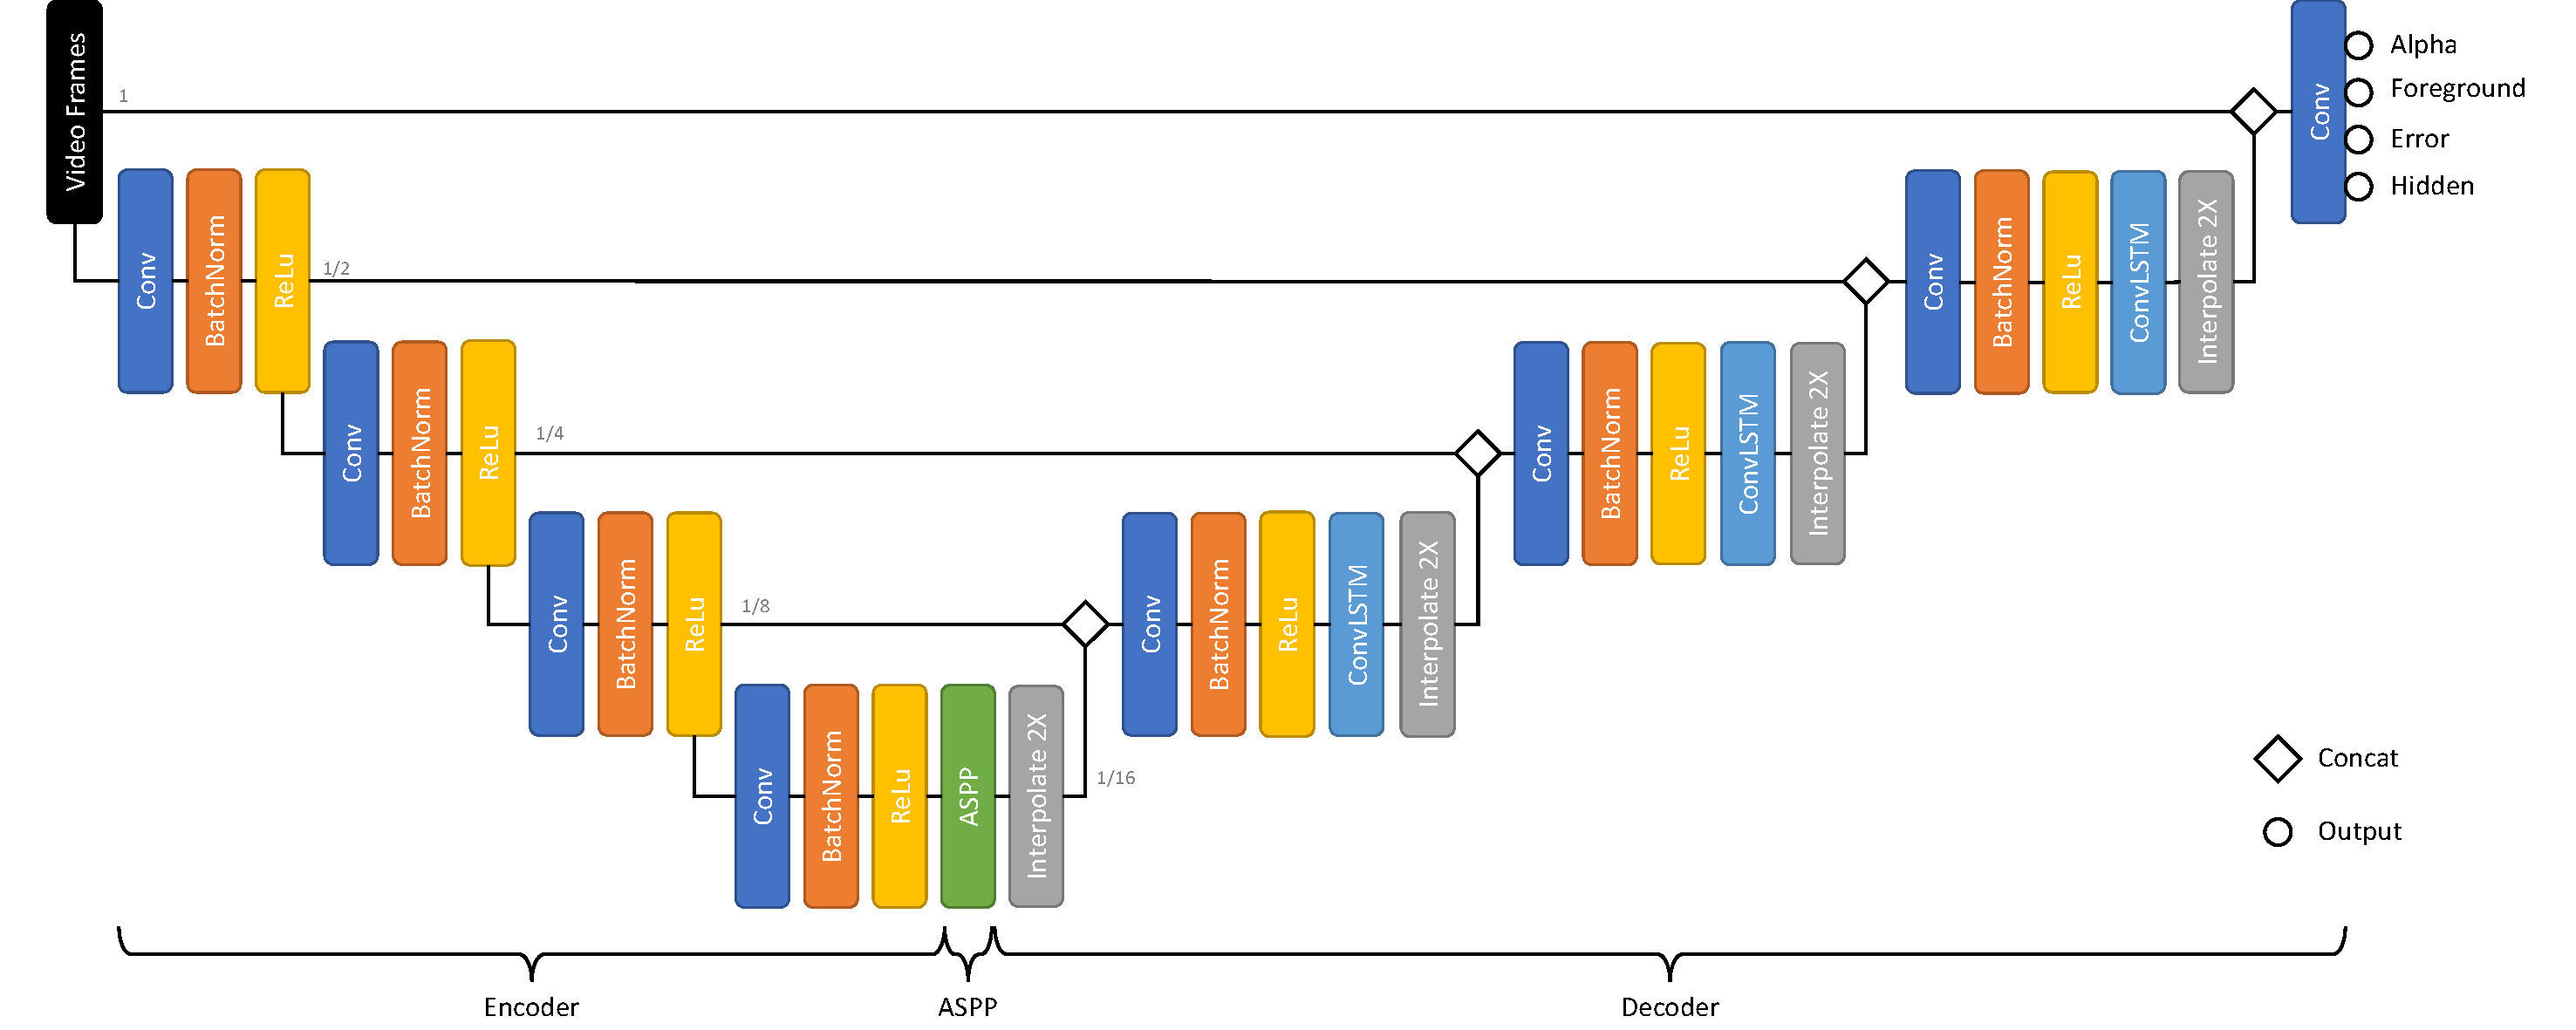
\includegraphics[width=1\textwidth]{img/modelConvLSTM.pdf}
    \end{center}
    \caption{The architecture of our network.}
    \label{modelConvLSTM}
\end{figure*}

\subsubsection{Encoder}

The Encoder consists of four encoder blocks (EB), each contains a convolutional layer, a batch normalization layer and a ReLU activation layer. This architecture is taken from ResNet50 pretrained on ImageNet. It is by design that after each EB, the size of feature maps halves, and the number of channels increases in the order $[3, 64, 256, 512, 2048]$.

\subsubsection{ASPP}

Atrous Spatial Pyramid Pooling (ASPP) utilizes the fusion of multiple convolutions with different dilation rates to increase receptive field, shrink the size of feature maps, just like pooling. But, meanwhile, it can keep more informative features.

\subsubsection{Decoder}

The decoder can be divided into three decoder blocks (DB) and an output block (OB), each of them starts with upsampling, implemented by 2x bilinear interpolation. Together with output of each EB, the feature map then pass a convolutional layer, a batch normalization layer, a ReLU activation layer and ConvLSTM layer. The output size of each DB doubles and the number of channels decreases in the order  $[768, 384, 128, 51, 37]$. The OB generates the output directly, which contains 37 channels. The first channel is Alpha, which is the matte in greyscale. The next 3 channels are Foreground, it is designed to make the model focus more on the foreground. The next channel is Error, it is the predicted error, which will then be compared with the error between the predicted alpha and the ground truth alpha. The rest channels are set for the refine part of \cite{linRealTimeHighResolutionBackground2020a}, which is not used in this project. But we still remain these channels for easier transfer learning.

\subsubsection{ConvLSTM}

\begin{equation}
    \begin{aligned}
        \mathbf{i}_{\mathbf{t}} & = \operatorname{Sigmoid}\left(\operatorname{Conv}\left(\mathbf{x}_{\mathbf{t}} ; \mathbf{w}_{\mathbf{x i}}\right)+\operatorname{Conv}\left(\mathbf{h}_{\mathbf{t}-\mathbf{1}} ; \mathbf{w}_{\mathbf{h i}}\right)+\mathbf{b}_{\mathbf{i}}\right)    \\
        \mathbf{f}_{\mathbf{t}} & = \operatorname{Sigmoid}\left(\operatorname{Conv}\left(\mathbf{x}_{\mathbf{t}} ; \mathbf{w}_{\mathbf{x f}}\right)+\operatorname{Conv}\left(\mathbf{h}_{\mathbf{t}-\mathbf{1}} ; \mathbf{w}_{\mathbf{h f}}\right)+\mathbf{b}_{\mathbf{f}}\right)    \\
        \mathbf{o}_{\mathbf{t}} & = \operatorname{Sigmoid}\left(\operatorname{Conv}\left(\mathbf{x}_{\mathbf{t}} ; \mathbf{w}_{\mathbf{x o}}\right)+\operatorname{Conv}\left(\mathbf{h}_{\mathbf{t}-\mathbf{1}} ; \mathbf{w}_{\mathbf{h o}}\right)+\mathbf{b}_{\mathbf{o}}\right)    \\
        \mathbf{g}_{\mathbf{t}} & = \operatorname{Tanh} \quad\left(\operatorname{Conv}\left(\mathbf{x}_{\mathbf{t}} ; \mathbf{w}_{\mathbf{x g}}\right)+\operatorname{Conv}\left(\mathbf{h}_{\mathbf{t}-\mathbf{1}} ; \mathbf{w}_{\mathbf{h g}}\right)+\mathbf{b}_{\mathbf{g}}\right) \\
        \mathbf{c}_{\mathbf{t}} & = \mathbf{f}_{\mathbf{t}} \odot \mathbf{c}_{\mathbf{t}-\mathbf{1}}+\mathbf{i}_{\mathbf{t}} \odot \mathbf{g}_{\mathbf{t}}                                                                                                                           \\
        \mathbf{h}_{\mathbf{t}} & = \mathbf{o}_{\mathbf{t}} \odot \operatorname{Tanh}\left(\mathbf{c}_{\mathbf{t}}\right)
    \end{aligned}
\end{equation}\label{convLSTM}


\subsection{Loss Function}

TODO

\section{Experiments}

TODO

\subsection{Experiment Setup}

\subsubsection{Datasets}

TODO

\subsubsection{Metrics}

TODO

\paragraph{MAD (mean absolute difference)}

TODO

\paragraph{MSE (mean squared error)}

TODO

\paragraph{GRAD (Gradient)}

TODO

\paragraph{CONN (Connectivity)}

TODO

\subsubsection{Implementation}

TODO

\subsection{Experiment Results}

TODO

\begin{table}
    \centering
    \caption{caption}
    \label{result}
    \begin{tabular}{lcccc}
        \toprule
        {}       & MAD              & MSE              & GRAD             & CONN               \\
        \midrule
        original & \textbf{2.04}    & \textbf{0.94}    & \textbf{0.11}    & \textbf{102.40}    \\
        \midrule
        transfer & 8.09             & 5.44             & \underline{6.73} & 406.09             \\
        convLSTM & \underline{5.18} & \underline{3.73} & 7.65             & \underline{259.67} \\
        \bottomrule
    \end{tabular}
\end{table}

\subsubsection{Comparing}

TODO

\subsubsection{Ablation Study}

TODO

\section{Conclusion}

Conclusion TODO

\cite{chenRethinkingAtrousConvolution2017}

\section{References}

\bibliographystyle{ieee_fullname}
\bibliography{reference}

\section{Review}

\subsection{Self Reflection}

TODO

\subsection{Confidential Peer Review}

TODO

In doing this project, to the best of my judgement,
I confirm that Jiahao Zhang mainly contributed to TODO,
and his/her overall contribution is about 34\%,
Peng Zhang mainly worked on TODO,
and his/her contribution is about 33\%,
and Hang Zhang was responsible for TODO,
and his/her contribution counts about 33\% of the total project workload.

\end{document}
